\documentclass{beamer}\usepackage[]{graphicx}\usepackage[]{color}
%% maxwidth is the original width if it is less than linewidth
%% otherwise use linewidth (to make sure the graphics do not exceed the margin)
\makeatletter
\def\maxwidth{ %
  \ifdim\Gin@nat@width>\linewidth
    \linewidth
  \else
    \Gin@nat@width
  \fi
}
\makeatother

\definecolor{fgcolor}{rgb}{1, 0.894, 0.769}
\newcommand{\hlnum}[1]{\textcolor[rgb]{0.824,0.412,0.118}{#1}}%
\newcommand{\hlstr}[1]{\textcolor[rgb]{1,0.894,0.71}{#1}}%
\newcommand{\hlcom}[1]{\textcolor[rgb]{0.824,0.706,0.549}{#1}}%
\newcommand{\hlopt}[1]{\textcolor[rgb]{1,0.894,0.769}{#1}}%
\newcommand{\hlstd}[1]{\textcolor[rgb]{1,0.894,0.769}{#1}}%
\newcommand{\hlkwa}[1]{\textcolor[rgb]{0.941,0.902,0.549}{#1}}%
\newcommand{\hlkwb}[1]{\textcolor[rgb]{0.804,0.776,0.451}{#1}}%
\newcommand{\hlkwc}[1]{\textcolor[rgb]{0.78,0.941,0.545}{#1}}%
\newcommand{\hlkwd}[1]{\textcolor[rgb]{1,0.78,0.769}{#1}}%
\let\hlipl\hlkwb

\usepackage{framed}
\makeatletter
\newenvironment{kframe}{%
 \def\at@end@of@kframe{}%
 \ifinner\ifhmode%
  \def\at@end@of@kframe{\end{minipage}}%
  \begin{minipage}{\columnwidth}%
 \fi\fi%
 \def\FrameCommand##1{\hskip\@totalleftmargin \hskip-\fboxsep
 \colorbox{shadecolor}{##1}\hskip-\fboxsep
     % There is no \\@totalrightmargin, so:
     \hskip-\linewidth \hskip-\@totalleftmargin \hskip\columnwidth}%
 \MakeFramed {\advance\hsize-\width
   \@totalleftmargin\z@ \linewidth\hsize
   \@setminipage}}%
 {\par\unskip\endMakeFramed%
 \at@end@of@kframe}
\makeatother

\definecolor{shadecolor}{rgb}{.97, .97, .97}
\definecolor{messagecolor}{rgb}{0, 0, 0}
\definecolor{warningcolor}{rgb}{1, 0, 1}
\definecolor{errorcolor}{rgb}{1, 0, 0}
\newenvironment{knitrout}{}{} % an empty environment to be redefined in TeX

\usepackage{alltt}
\usepackage{../371g-slides}
\usepackage{preview}
\title{Interactions 2}
\subtitle{Lecture 16}
\author{STA 371G}
\IfFileExists{upquote.sty}{\usepackage{upquote}}{}
\begin{document}
  
  

  \frame{\maketitle}

  % Show outline at beginning of each section
  \AtBeginSection[]{ 
    \begin{frame}<beamer>
      \tableofcontents[currentsection]
    \end{frame}
  }

  %%%%%%% Slides start here %%%%%%%

  \begin{darkframes}
    %\begin{frame}{Project}
    %  \begin{itemize}
    %    \item It's time to start thinking about our final project!
    %  \end{itemize}
    %\end{frame}

    \begin{frame}{NBA data}
      Basketball-Reference.com provides detailed data on NBA teams and players. We'll look at team data for 4 seasons ending in 2016; each of these metrics is the average across the season:
      \begin{itemize}
        \item \textbf{PTS}: Total points
        \item \textbf{PCT3P}: Percentage of 3-point shots made
        \item \textbf{N3PA}: Number of 3-point shots attempted
      \end{itemize}
      There are 30 NBA teams $\times$ 4 seasons = 120 cases in this file.
    \end{frame}

    \begin{frame}{NBA data}
      In basketball, there are three ways to score:
      \begin{columns}[onlytextwidth]
        \column{.6\textwidth}
          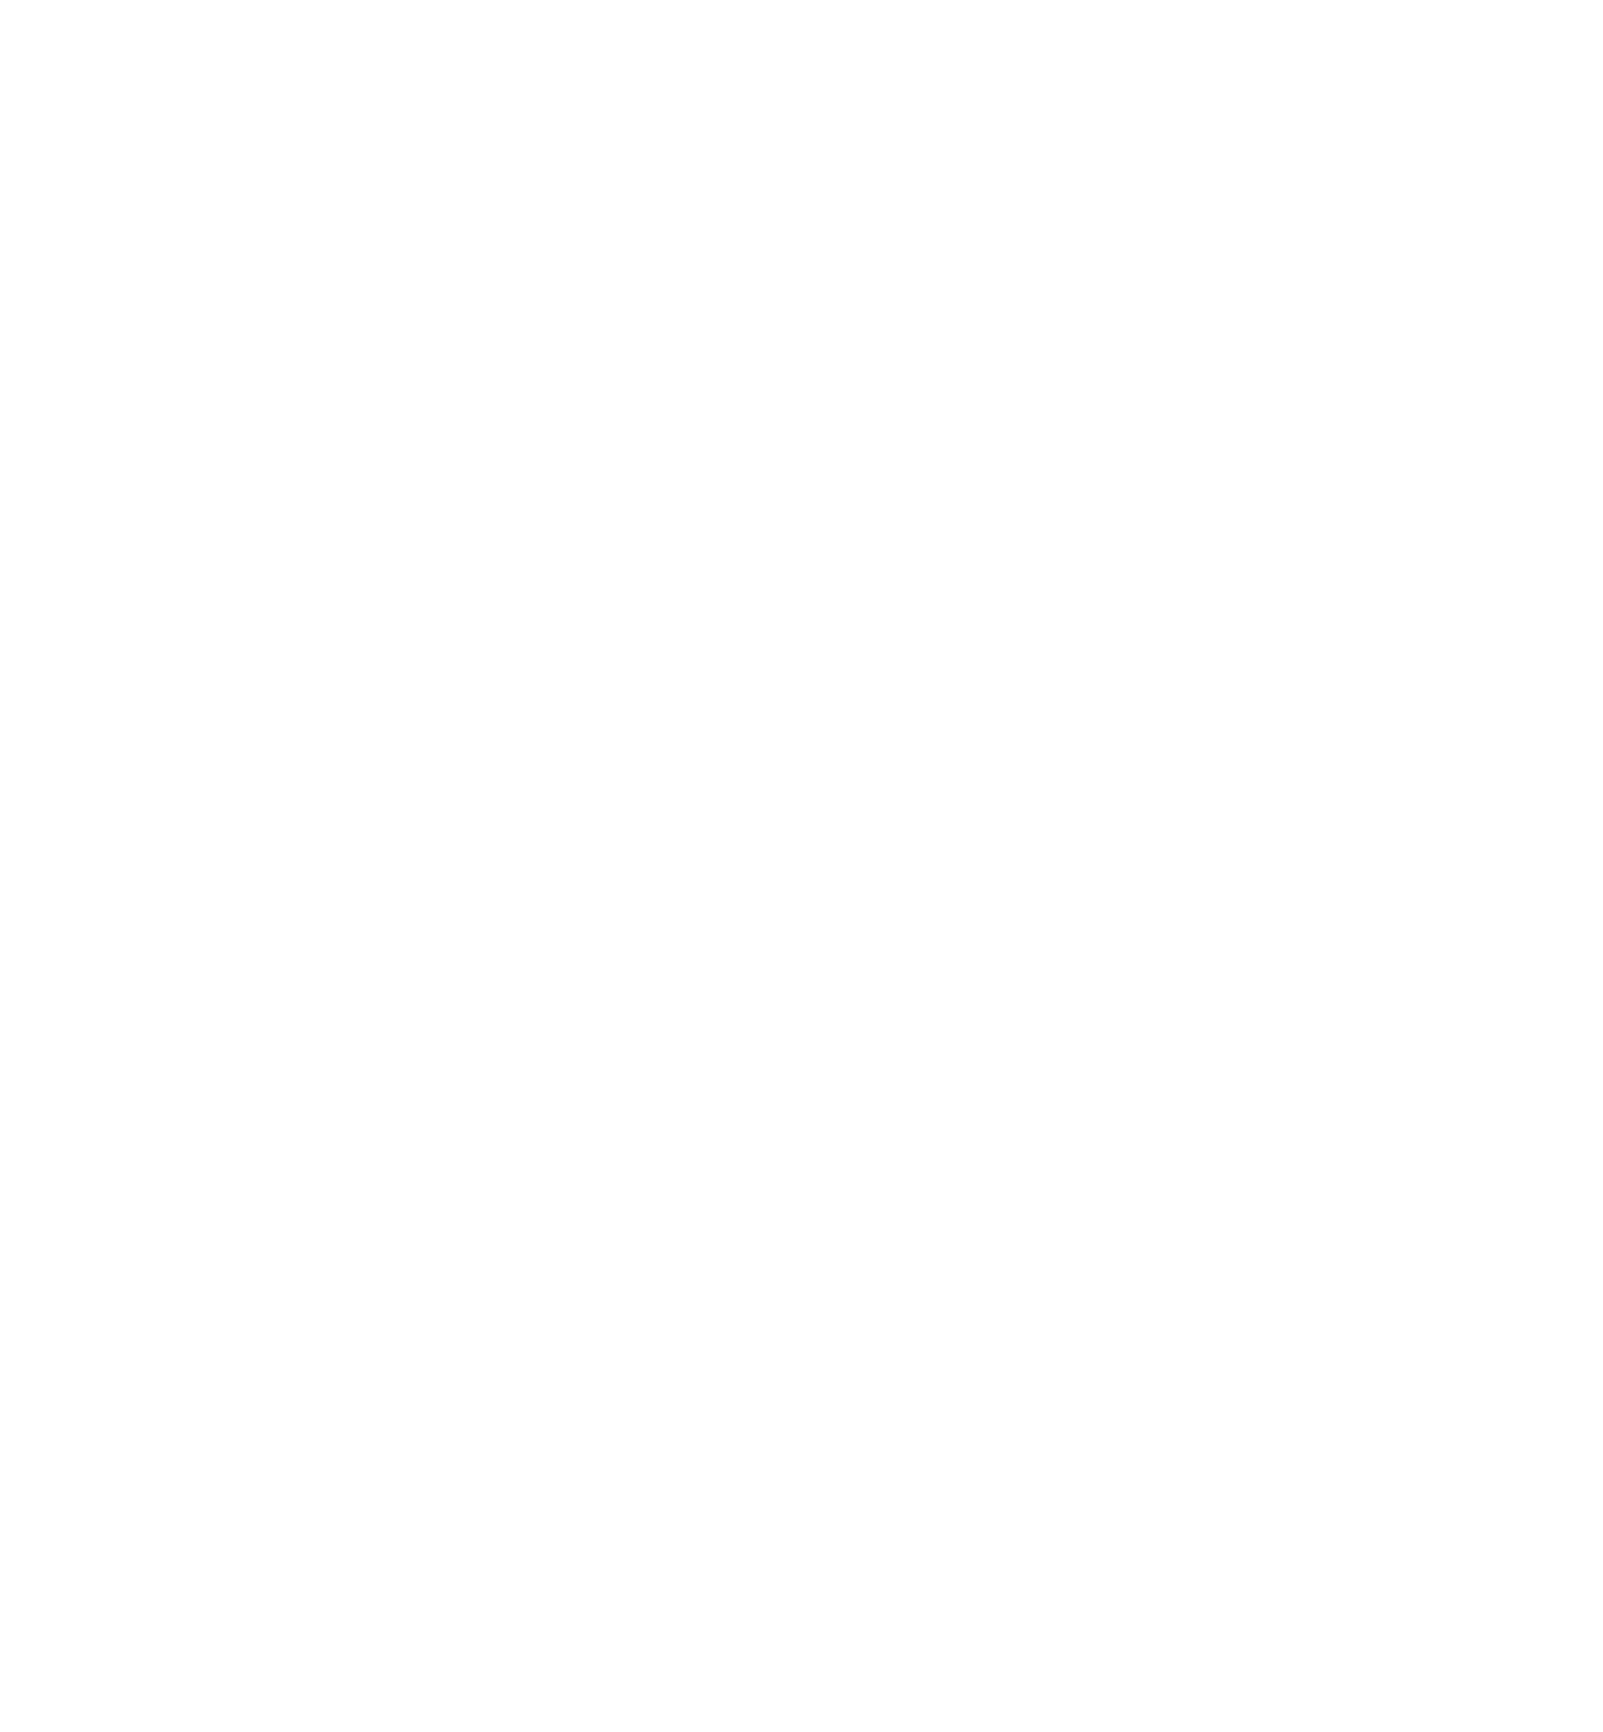
\includegraphics[width=\textwidth]{basketball-court.png}
        \column{.4\textwidth}
          \begin{itemize}
            \item \textbf{1 point} for free throws made after a foul by the other team
            \item \textbf{2 points} for shots made inside the 3-point line
            \item \textbf{3 points} for shots made outside the 3-point line
          \end{itemize}        
      \end{columns}
    \end{frame}

\begin{frame}[fragile]
\begin{knitrout}
\definecolor{shadecolor}{rgb}{0.137, 0.137, 0.137}\begin{kframe}
\begin{alltt}
\hlkwd{plot}\hlstd{(nba}\hlopt{$}\hlstd{N3PA, nba}\hlopt{$}\hlstd{PTS,} \hlkwc{pch}\hlstd{=}\hlnum{16}\hlstd{,} \hlkwc{col}\hlstd{=}\hlstr{'orange'}\hlstd{,}
  \hlkwc{xlab}\hlstd{=}\hlstr{'Num 3-point shots attempted'}\hlstd{,} \hlkwc{ylab}\hlstd{=}\hlstr{'Total points'}\hlstd{)}
\end{alltt}
\end{kframe}
\input{/tmp/figures/unnamed-chunk-2-1.tikz}

\end{knitrout}
      \lc
\end{frame}

\begin{frame}[fragile]
      \fontsize{8}{8}\selectfont
\begin{knitrout}
\definecolor{shadecolor}{rgb}{0.137, 0.137, 0.137}\begin{kframe}
\begin{alltt}
\hlstd{model1} \hlkwb{<-} \hlkwd{lm}\hlstd{(PTS} \hlopt{~} \hlstd{N3PA,} \hlkwc{data}\hlstd{=nba)}
\hlkwd{summary}\hlstd{(model1)}
\end{alltt}
\begin{verbatim}

Call:
lm(formula = PTS ~ N3PA, data = nba)

Residuals:
     Min       1Q   Median       3Q      Max 
-11.2454  -2.5114   0.0549   2.2252   8.6405 

Coefficients:
            Estimate Std. Error t value Pr(>|t|)    
(Intercept) 86.19204    1.77464  48.569  < 2e-16 ***
N3PA         0.64842    0.07935   8.171 3.89e-13 ***
---
Signif. codes:  0 '***' 0.001 '**' 0.01 '*' 0.05 '.' 0.1 ' ' 1

Residual standard error: 3.496 on 118 degrees of freedom
Multiple R-squared:  0.3614,	Adjusted R-squared:  0.356 
F-statistic: 66.77 on 1 and 118 DF,  p-value: 3.889e-13
\end{verbatim}
\end{kframe}
\end{knitrout}
      \lc
\end{frame}

    \begin{frame}{Can we do better?}
      \begin{center}
        $R^2=36\%$, so we can explain
        36\% of the variance in total points based only on
        knowing the number of 3-point attempts.

        \pause\bigskip

        This means that \textbf{most} of the variance (64\%) in total points is \textbf{not} explained by the number of 3-point attempts.

        \pause\bigskip

        Let's add another variable to our model --- why might 3-point percentage be useful as another predictor?
      \end{center}
      \lc
    \end{frame}
    
\begin{frame}[fragile]{Can we do better?}
      \fontsize{8}{8}\selectfont
\begin{knitrout}
\definecolor{shadecolor}{rgb}{0.137, 0.137, 0.137}\begin{kframe}
\begin{alltt}
\hlstd{model2} \hlkwb{<-} \hlkwd{lm}\hlstd{(PTS} \hlopt{~} \hlstd{N3PA} \hlopt{+} \hlstd{PCT3P,} \hlkwc{data}\hlstd{=nba)}
\hlkwd{summary}\hlstd{(model2)}
\end{alltt}
\begin{verbatim}

Call:
lm(formula = PTS ~ N3PA + PCT3P, data = nba)

Residuals:
    Min      1Q  Median      3Q     Max 
-8.3487 -2.1392 -0.0791  1.8691  9.1904 

Coefficients:
            Estimate Std. Error t value Pr(>|t|)    
(Intercept) 62.00493    5.61396  11.045  < 2e-16 ***
N3PA         0.56467    0.07587   7.442 1.82e-11 ***
PCT3P        0.73415    0.16292   4.506 1.57e-05 ***
---
Signif. codes:  0 '***' 0.001 '**' 0.01 '*' 0.05 '.' 0.1 ' ' 1

Residual standard error: 3.241 on 117 degrees of freedom
Multiple R-squared:  0.4558,	Adjusted R-squared:  0.4465 
F-statistic:    49 on 2 and 117 DF,  p-value: 3.478e-16
\end{verbatim}
\end{kframe}
\end{knitrout}
      \lc
\end{frame}

    \begin{frame}{Can we do even better?}
      \begin{center}
        It would make sense that the \textbf{impact} of the number of 3-pointers taken on total points would \textbf{depend on} how well the team shoots the 3!

        \pause\bigskip

        This sounds like an interaction --- let's make a model with an interaction between the two predictors!
      \end{center}
    \end{frame}
    
\begin{frame}[fragile]
      \fontsize{8}{8}\selectfont
\begin{knitrout}
\definecolor{shadecolor}{rgb}{0.137, 0.137, 0.137}\begin{kframe}
\begin{alltt}
\hlstd{model3} \hlkwb{<-} \hlkwd{lm}\hlstd{(PTS} \hlopt{~} \hlstd{N3PA} \hlopt{*} \hlstd{PCT3P,} \hlkwc{data}\hlstd{=nba)}
\hlkwd{summary}\hlstd{(model3)}
\end{alltt}
\begin{verbatim}

Call:
lm(formula = PTS ~ N3PA * PCT3P, data = nba)

Residuals:
    Min      1Q  Median      3Q     Max 
-7.2629 -2.2757  0.1148  1.9698  9.3756 

Coefficients:
             Estimate Std. Error t value Pr(>|t|)    
(Intercept) 122.84903   30.58937   4.016 0.000105 ***
N3PA         -2.11904    1.32903  -1.594 0.113561    
PCT3P        -0.98410    0.86465  -1.138 0.257400    
N3PA:PCT3P    0.07561    0.03739   2.023 0.045423 *  
---
Signif. codes:  0 '***' 0.001 '**' 0.01 '*' 0.05 '.' 0.1 ' ' 1

Residual standard error: 3.199 on 116 degrees of freedom
Multiple R-squared:  0.4743,	Adjusted R-squared:  0.4608 
F-statistic: 34.89 on 3 and 116 DF,  p-value: 3.798e-16
\end{verbatim}
\end{kframe}
\end{knitrout}
\end{frame}

\begin{frame}[fragile]

      Model 3 corresponds to the regression equation
      \[
        \widehat{\text{PTS}} = 122.85 
          - 2.12 \cdot\text{N3PA}
          - 0.98 \cdot\text{PCT3P}
          + 0.08 \cdot\text{N3PA}\cdot\text{PCT3P}.
      \]

      \pause

      We interpret the coefficients as follows:
      \begin{itemize}[<+->]
        \item \textbf{Intercept} (122.85) is our prediction of total points when $\text{N3PA}=\text{PCT3P}=0$. (Meaningless in this context!)
        \item \textbf{N3PA} ($-2.12$) is the predicted increase in total points for each additional 3-pointer taken, when $\text{PCT3P}=0$.
        \item \textbf{PCT3P} ($-0.98$)  is the predicted increase in total points for each additional percentage point of 3-point shooting accuracy, when $\text{N3PA}=0$.
        \item \textbf{$\text{N3PA}\cdot\text{PCT3P}$} ($0.08$) can be interpreted in two ways:\pause
          \begin{itemize}[<+->]
            \item the increase in the \emph{slope coefficient} for N3PA for each 1-unit increase of PCT3P.
            \item the increase in the \emph{slope coefficient} for PCT3P for each 1-unit increase of N3PA.
          \end{itemize}
      \end{itemize}
      \lc
\end{frame}

    \begin{frame}
\begin{knitrout}
\definecolor{shadecolor}{rgb}{0.137, 0.137, 0.137}
\input{/tmp/figures/unnamed-chunk-7-1.tikz}

\end{knitrout}
    \end{frame}

    \begin{frame}
\begin{knitrout}
\definecolor{shadecolor}{rgb}{0.137, 0.137, 0.137}
\input{/tmp/figures/unnamed-chunk-8-1.tikz}

\end{knitrout}
    \end{frame}

    \begin{frame}
\begin{knitrout}
\definecolor{shadecolor}{rgb}{0.137, 0.137, 0.137}
\input{/tmp/figures/unnamed-chunk-9-1.tikz}

\end{knitrout}
      \lc
    \end{frame}
\begin{frame}
\[
        \widehat{\text{PTS}} = 122.85 
          - 2.12 \cdot\text{N3PA}
          - 0.98 \cdot\text{PCT3P}
          + 0.08 \cdot\text{N3PA}\cdot\text{PCT3P}.
      \]

\begin{itemize}
\item How many points per game do you predict for a team that shoots 3-pointers at the NBA average rate (35.4) and that takes 30 3-pointers per game?
\pause
\item How bad would a team have to shoot the 3 before taking 3-point shots start to have a negative impact on total points?
\end{itemize}
\end{frame}

    \begin{frame}
\begin{knitrout}
\definecolor{shadecolor}{rgb}{0.137, 0.137, 0.137}
\input{/tmp/figures/unnamed-chunk-10-1.tikz}

\end{knitrout}
      \lc
    \end{frame}

  \end{darkframes}

  \end{document}
